\documentclass[a4paper,12pt]{article}
\usepackage{graphicx}
\usepackage{amsmath, amsfonts}
\usepackage{amssymb}

\usepackage[utf8x]{inputenc}
\usepackage[T1]{fontenc}

\usepackage{lmodern}
\usepackage{textcomp}

\usepackage{natbib}

\usepackage[top=1.2in,bottom=1.2in,left=3.cm,right=3.cm,a4paper]{geometry}

\usepackage[font=footnotesize]{caption}

\usepackage{xcolor}

%\usepackage{hyperref}

%\hypersetup{
%    colorlinks,
%    linkcolor={red!50!black},
%    citecolor={blue!50!black},
%    urlcolor={blue!99!black}
%}

\usepackage{titling}

\pretitle{%

\includegraphics[width=0.3\linewidth]{../fig/logo_UGA}
\hspace{5cm}

\includegraphics[width=0.3\linewidth]{../fig/logo_IGE}
\vspace{2cm}
\begin{center}
\LARGE
}
\posttitle{\end{center}}
\postdate{\par\end{center}\vspace{12cm}~}

\usepackage[nottoc,numbib]{tocbibind}

%%%%%%%%%%%%%%%%%%%%%%%%%%%%%%%%%%%%%%%%%%%%%%%%%%%%%%%%
\title{Numerical experiments of glacial inceptions in Northern Europe}
\author{Ruben ESPELETA BOLIVAR}

% to define new commands
\newcommand{\R}{\mathcal{R}}
\newcommand{\mean}[1]{\langle #1 \rangle}

% to show the pieces of advice
\newcommand{\advice}[1]{{\it #1}}
% to hide the pieces of advice
% \newcommand{\advice}[1]{}

\begin{document}

\renewcommand{\labelitemi}{$\bullet$}

\maketitle

\tableofcontents

\newpage

\begin{abstract}
	This is the abstract part
\end{abstract}
\pagebreak
\section{Introduction}

Glaciers and ice sheets dinamics play a vital role in the global oceanic and climatic systems. In Antarctica, for example, cold water is formed and because freshwater ice at the surface freezes into icebergs, the water is not only cold, but salty. This cold, dense, salty water sinks into the ocean floor, and drives the global ocean currents, being replaced with warmer surface water from the equatorial regions. This is known as the global thermohaline circulation, and these ocean currents drive the earth's climatic system (insertar referencia de la pagina).

Historically, this type of climatic system and processes has been affected by climate change. Water melting from glaciers has the potential to raise sea levels (insertar referencia pagina) and global warming causes this melting of ice caps. If all the ice were to melt completely, the sea level would rise by an estimated 65m \cite[]{morlighem2017bedmachine,haywood2011pliocene} and force populations to emigrate their land submerged by water. This may be an indication of how impactfull could be the climate change in the future.

In order to understand these impacts and the influence that climate change has over the dynamics and melting of ice sheets and glaciers, numerical models are developped. Through these models based on finite elements, we can have simulations that can make better predictions of future ice sheets behaviour and rate of sea level rise, and ultimately provide policy makers with improved estimates of future change.

\begin{figure}[!h]
	\centering
	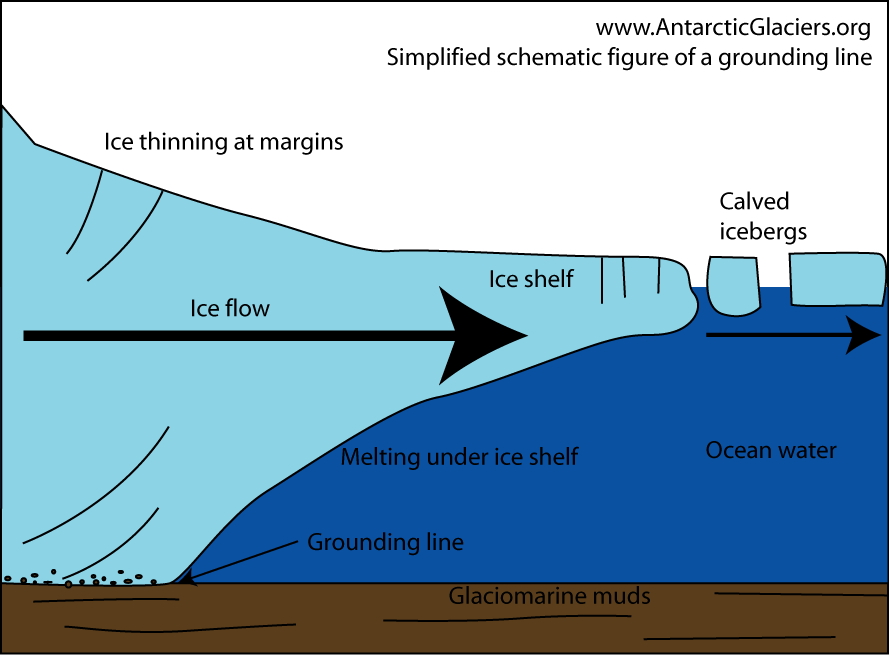
\includegraphics[width=0.7\linewidth]{../fig/groundingline}
	\caption{Simplified schematic of a tributary glacier feeding into an ice shelf, showing the grounding line (where the glacier begins to float).}
	\label{groundingline}
\end{figure}

However, understanding the influence of global warming and climate change on the behaviour of glaciers and ice sheets, involves the challenge of understanding how the different parameters and variables that can affect the ice sheet melting are related, and the role they play in the dynamics of the glaciers. One of this important parameters is the grounding line. Glaciers that end in the ocean are cold tidewater glaciers. They may be grounded (the glacier is in contact with the bed entirely), or parts of the glacier terminus may be flotating. Glaciers that flow into an ice shelf are called tributary glaciers (referencia de la pagina) as the one shown in figure \ref{groundingline}. The point at which  glaciers and ice shelves start to flow is the grounding line. The location of the grounding line is important, because mass loss from glaciers is strongly linked to changes in the ice shelves and their grounding lines \cite[]{brunt2010mapping,pritchard2012antarctic}. Changes in the grounding line can result in very rapid changes in glacier and ice-shelf behaviour.

During this project, the main objective is to understand the direct impact of changes in the position of the grounding line on the flow dynamics of ice sheets glaciers using the finite element model Elmer/Ice as a simulation tool, using different spatial resolutions to compare the different changes in position of the grounding line obtained by these numerical methods approximations, and we will test the ability of this model to predict the position of the grounding line.
\section{Context, social and scientific issues}
\subsection{Context}

Almost all Antarctica is covered in Ice. Less than 1\% its land area is ice free.This means that, across Antarctica, almost all glaciers end in the ocean, whereupon they calve icebergs. These glaciers can be grounded, or can end in flotating ice tongues or larger ice shelves (figure \ref{groundingline}). These flotating ice shelves move with the tide. Ice shelves fringe 75\% of Antarctica's coastline, while collecting 20\% of its snowfall over 11\% of its area \cite[]{rignot2013ice}.

The transition from grounded ice sheets to flotating ice shelf plays an important role in controlling marine ice sheet dynamics, as it determines the rate at which ice flows out of the grounded part of the ice sheet \cite[]{schoof2007ice}. This is because ice flux through the grounding line increases sharply with ice thickness at the grounding line. This means that grounding lines are unstable on reverse-bed slopes, such as those under Pine island glacier, because recession into deeper water increases ice flux and further encourages more glacier recession (insertar bibliografia de pagina).

Grounding lines are actually more of a zone. The grounding zone is the region where ice transitions from grounded ice sheet to freely flotating ice shelf, typically over several kilometers. The floating ice shelf changes in elevation in response to tides, atmospheric air, pressure and oceanic processes. Grounding occurs when the ice shelf comes into contact with the bedrock below (insertat cita pagina).

The grounding zone is the region between point F on figure \ref{groundingzone}, where there is no tidal movement, and point H, which is the seaward limit of ice flexure, where the ice is free-floating.

\begin{figure}[!h]
	\centering
	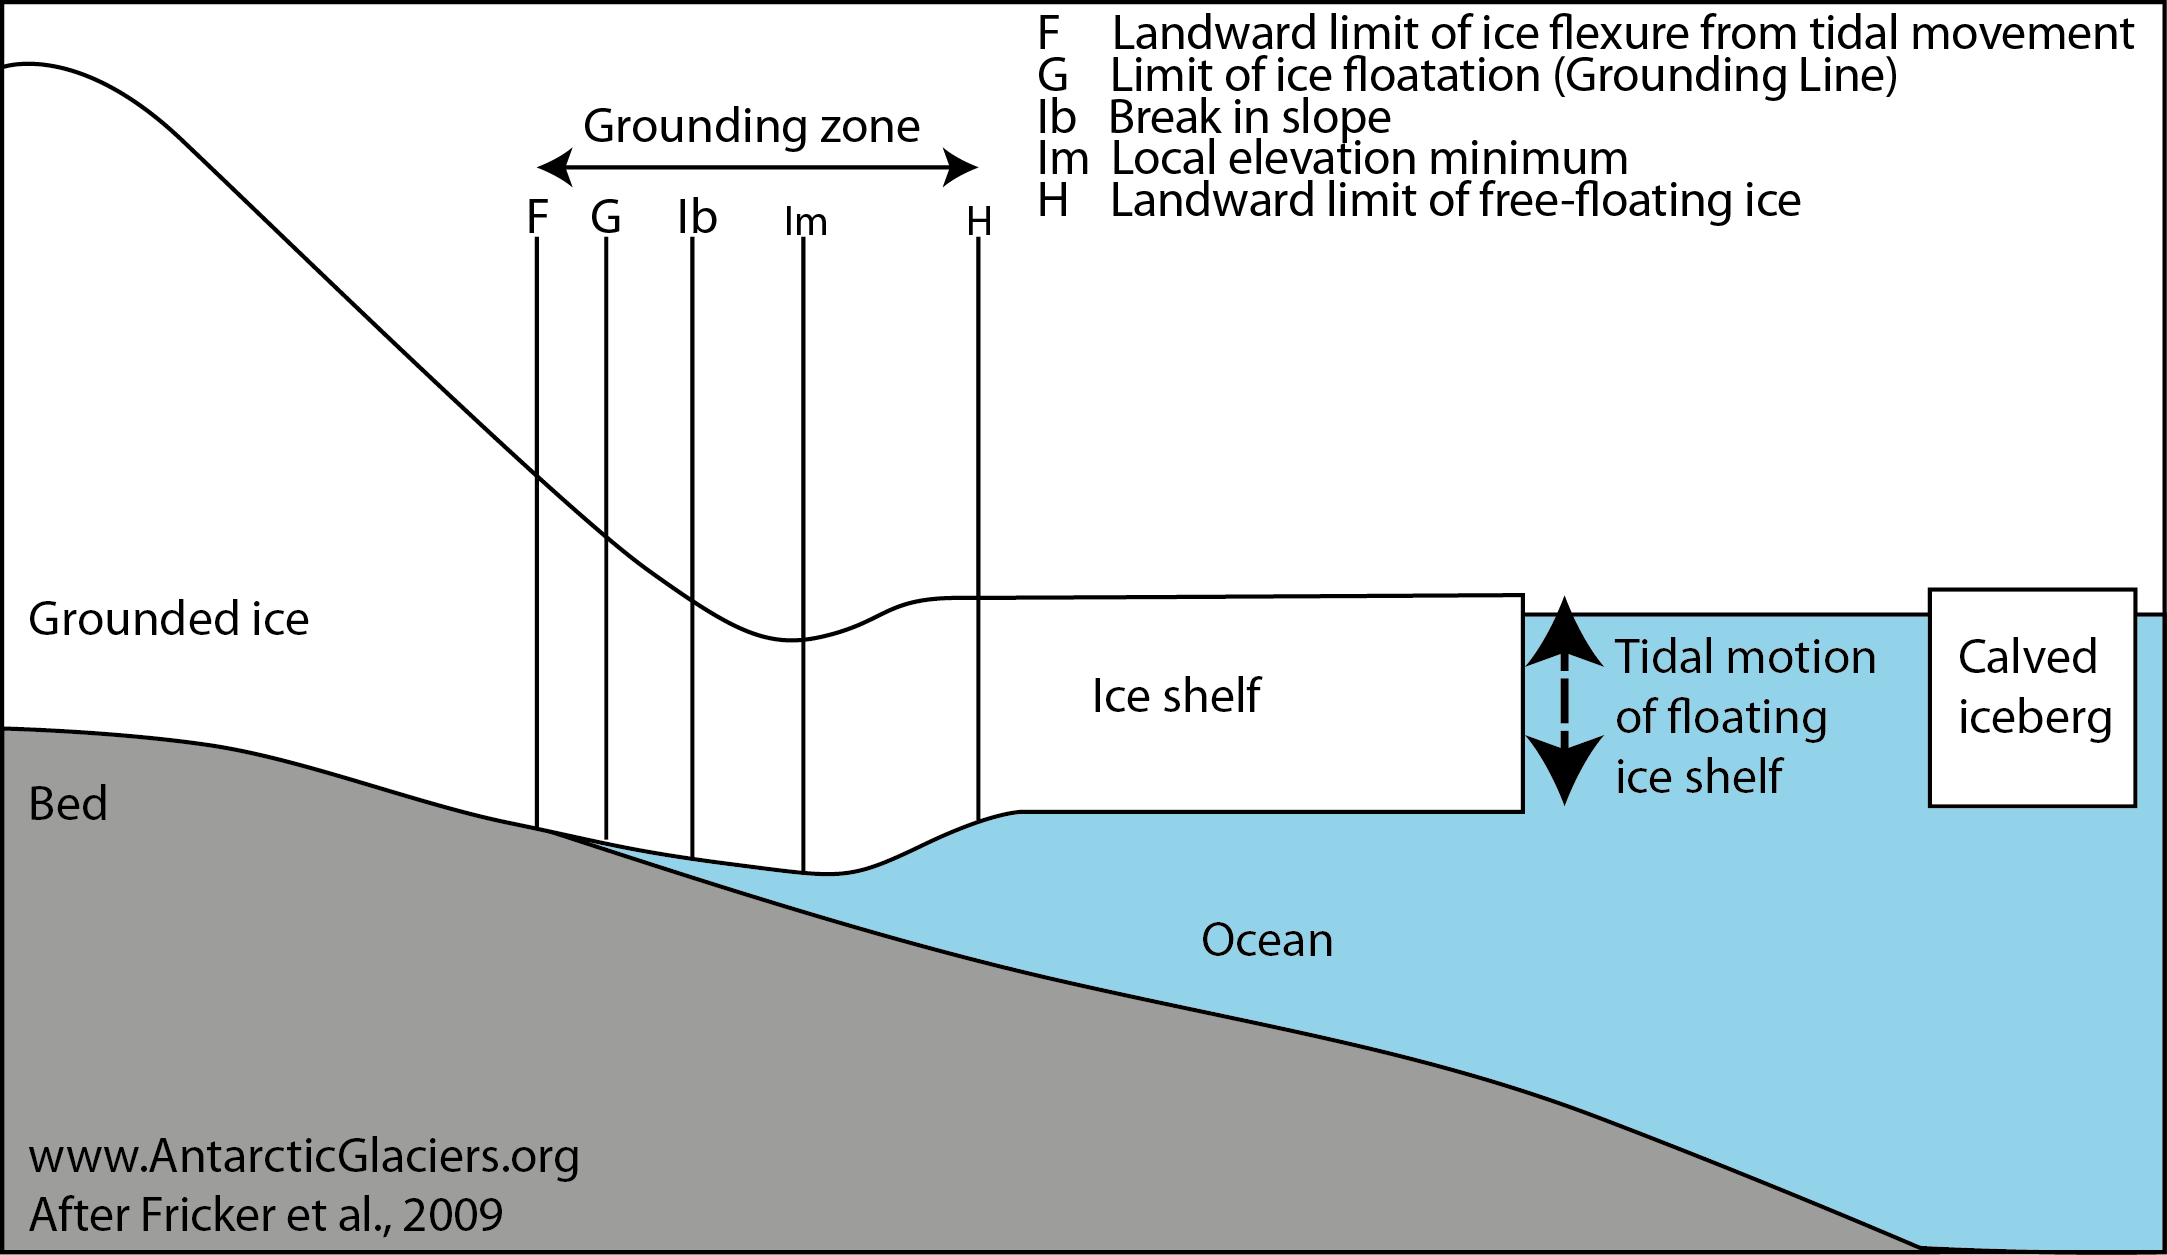
\includegraphics[width=0.7\linewidth]{../fig/groundingzone}
	\caption{Grounding zone \cite[]{fricker2009mapping}.}
	\label{groundingzone}
\end{figure}


\subsection{Social and scientific issues}

The Antarctic continent is drained by numerous large ice streams. They have considerable variability at short (sub-decadal) timescales, with recent observations of thinning, acceleration, deceleration, lateral migration and stagnation \cite[]{livingstone2012antarctic}. The mechanisms controlling these variations and advance and recession of grounding lines include a number of potential forcings, such as oceanic temperatures, sea level changes, air temperature, ocean tides, subglacial bathymetry, geomorphological features, subglacial meltwater, thermodynamics, and the size of the drainage basin \cite[]{livingstone2012antarctic}.

Around the Antartic peninsula, a number of ice shelves have recently dramatically collapsed \cite[]{cook2010overview,scambos2009ice}, resulting in glacier acceleration, thinning and grounding line retreat \cite[]{pritchard2007widespread,rignot2004accelerated}. In fact, Antarctic ice shelves appear crucial to the stability of their tributary glaciers \cite[]{pritchard2012antarctic}, and melting ice shelves could have catastrophic consequences for many glaciers. This is particularly concerning for the West Antartic Ice sheet, which is largely grounded below see level \cite[]{lythe2001bedmap}, and removal of this could raise sea levels by 3.3m \cite[]{bamber2009reassessment,mercer1978west}.

The grounding zone can be difficult to detect; it may take place over a wide area \cite[]{fricker2009mapping}, and this area can be remote and inaccessible and so difficult to monitor. Fortunately, there is a subtle feature that can be observed on satellite images. There is often an elevation minimum between points G and H shown in figure \ref{groundingzone}. Elevation profiles across the grounding line will often show a break in slope (point lb in figure \ref{groundingzone}). 

Other methods for detecting the grounding line rely on measuring changes in surface elevation during the tydal cycle, which can be measured by GPS or satellite synthetic aperture radar \cite[]{rignot2011antarctic,fricker2009mapping,brunt2010mapping}.

\section{State of the art}
Marine ice sheets rest on beds that lie below sea level and their drainage takes place through surrounding ice shelves. Grounded ice-sheet flow is dominated by horizontal shearing while the ice-shelf flow is dominated by longitudinal stretching and lateral shearing \cite[]{durand2009full}. The two types of flow couple together across a transition zone near the grounding line, where longitudinal and shear stresses are of the same order of magnitude. A long debate on the dynamics of such ice sheets was initiated in the 1970s, when \cite{weertman1974stability} proposed that a marine ice sheet which lies on an upward-sloping bed is unstable. Recently, the instability hypothesis has been strongly reinforced, based on a boundary-layer theory due to \cite{schoof2007ice}. Moreover, \cite{vieli2005assessing} showed that the poor ability of marine ice-sheet models to give consistent prognostic results and, more particularly, they highlighted the influence of the grid size on model results. One of their main conclusions was that no reliable model was able to predict grounding line dynamics at the time of their study.

As a consequence, there is an urgent need to improve marine ice-sheets models in order to corroborate recent theoretical predictions, and to obtain confident simulations of the grounding line dynamics. \cite{durand2009marine} recently proposed a full stokes resolution of the ice-sheet/ice-shelf transition. This approach has been built on literature dealing with the coupling between a grounded ice sheet and a floating ice shelf and identyfing this transition zone as a crucial control of the marine ice sheet dynamics \cite[]{weertman1974stability,van1985response,chugunov1996modelling,hindmarsh1996stability,vieli2005assessing,schoof2007ice,schoof2007marine}.

Also, \cite{durand2009full} showed, using the finite element code Elmer, that the full stokes modeling of the ice-sheet/ice-shelf transition they proposed can give consistent predictions of grounding-line migration, and that their approach is highly sensitive to the chosen mesh resolution. However, in their results with a grid size down $<5 km$ in the vicinity of the grounding line, predictions start to be robust because: whatever the grid size($<5km$) the steady-state grounding line position is sensibly the same (6km the standart deviation), and with a grid-size refinement in the vicinity of the grounding line (200m), the steady state solution is independent of the applied perturbation in fluidity, provided this perturbation remains monotonic.

A comparison between the numerics and simulation results for the two full stokes ice sheet models FELIX-S \cite[]{leng2012parallel} and Elmer/Ice \cite[]{gagliardini2013capabilities} was presented by \cite{zhang2017comparison} and were applied to the marine ice sheet model intercomparison project for plan view models MIS-MIP3d. Both models gave similar results for the diagnostic experiment when using identical geometries and computational meshes, which can be interpreted as an indication of similarities between the two models. However, for other prognostic experiments, \cite{zhang2017comparison} found that FELIX-S grounding lines are relatively more retreated; results that are consistent with minor differences observed in the diagnostic experiment results and that \cite{zhang2017comparison} showed to be due to different choices in the implementation of basal boundary conditions in the two models (Figure \ref{comparison}). They also showed that these differences decrease with increasing horizontal grid resolution and that grounding-line positions for FELIX-S and Elmer/ice converge to within the estimated truncation error for Elmer/ice, and they proposed that an alternative estimate for the uncertainaty in the grounding line position is the span of grounding line position predicted by multiple stokes models. 

\begin{figure}[!h]
	\centering
	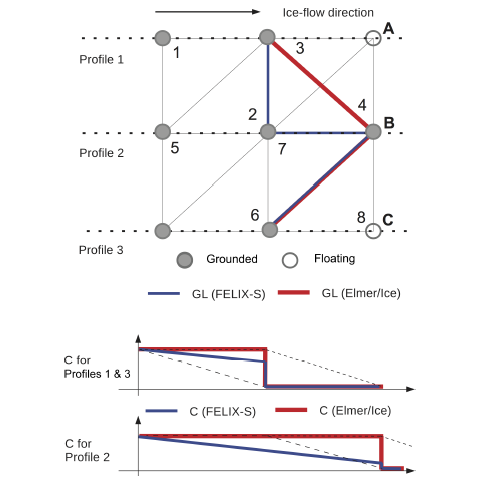
\includegraphics[width=0.7\linewidth]{../fig/comparison}
	\caption{A schematic of the different basal boundary masking schemes used by the two models.}
	\label{comparison}
\end{figure}

As shown in figure \ref{comparison}, circles denote the nodes at the ice-bed interface, defining the basal finite element faces (triangular and quadrilateral for FELIX-S and Elmer/Ice, respectively); open circles denote floating nodes for which $z(x,y,t)>b(x,y)$, and solid circles denote grounded nodes for which $z(x,y,t)=b(x,y)$ and $-\sigma_n>P_w$. As found by \cite{zhang2017comparison}, the different masking schemes lead to different grounding line positions and also to the different nodal values of C along profiles 1-3, as it is shown in figure \ref{comparison}.


\section{Scientific program}
\subsection{Methodology and tools}
\subsubsection{Ice sheet flow and modelling}
An ice sheet is a continuous sheet of land ice that covers a very large aream of several thousands to millions of squared meters. It is formed by an accumulation of snow which will densify under its own weight, until it becomes ice. This ice will then flow downhill under its weight, and can eventually reach the sea. If it does, and the ice propagates above the sea, this part of the ice sheet is called and ice shelf. The figure shows a diagram of an ice sheet showing different parts of it, such as the ice shelf, and some phenomena happening inside of it, such as the ice flow or the snow accumulation.

The ice is considered as a very viscous fluid, flowing on large time scales. The ice flow equations are then derived from the Stokes equation:
\begin{equation}
	div\sigma + \rho g = div\tau - gradp + \rho g = 0;
\end{equation}
with $\sigma$ the stress tensor, $\rho$ the density of the ice, g the gravity vector, $\tau$ the deviatoric stress tensor, with $\sigma = \tau - pI$ and $p=\frac{tr\sigma}{3}$. 

And the mass conservation:
\begin{equation}
	\frac{dh}{dt}+ div(uH)=M_s + M_b;
\end{equation}
With $u$ the velocity, H the ice thickness, $M_s$ and $M_b$ the mass balance at the surface and at the bottom respectively. $M_s$ will be defined, and $M_b$ is considered as 0 for convenience purposes. 

The stresses are related to the viscosity and the strain by the Glen's law:
\begin{equation}
	\tau = 2\eta\dot{\epsilon}
\end{equation}
With the viscosity that can be inferred according to \cite{gagliardini2013capabilities} as:
\begin{equation}
	\eta = \frac{1}{2}(EA)^\frac{-1}{n} \dot{\epsilon_e}^\frac{(1-n)}{n};
\end{equation}
Where:
\begin{itemize}
	\item The strain rate $\dot{\epsilon}$;
	\item Glen's constant n=3;
	\item The enhancement factor to account for an anisotropic effect E=1;
	\item The rheological parameter A=15,46;
\end{itemize}
For an ice sheet, the ratio of the vertical lenght over the horizontal lenght is a little more than $\frac{1}{10^3}$. Indeed, the thickness of an ice sheet is comprised between 0 to a few thousands of meters (e.g. the ice sheet in Greenland is 3300 m thick at most \cite[]{bamber2001new}) and typical horizontal lenght of an ice sheet is of the order of magnitude of 1000 km. This allows simplifications in the equations. One of them is the shallow ice approximation. It assumes a large ratio of horizontal to vertical lenght, that the basal shear stress is balanced by  the gravitational driving stress, and a large vertical to horizontal stress ratio. That represents a slow flow in the interior of an ice sheet (blue regions in Figure \ref{velocityglaciar}). The approximation makes the method computationally cheap and works well over long simulations.

\begin{figure}[!h]
	\centering
	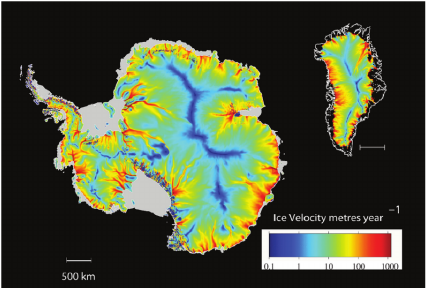
\includegraphics[width=0.7\linewidth]{../fig/velocityglaciar}
	\caption{Ice velocities in Antarctica and Greenland form. \cite[]{allison2009ice}.}
	\label{velocityglaciar}
\end{figure}
Figure \ref{velocityglaciar} shows a map of velocities in Antarctica and Greenland. Where this velocity is the highest, the basal shear stress cannot be considered as balanced by the gravity anymore. Instead, it is taken as 0 and the longitudinal stress dominates. This is the Shallow Shelf approximation, initially developed for ice shelves, but which has been extended to dragging ice streams. It is a 2D vertically integrated model, the ice velocity being depth-averaged.

But these approximations are not mandatory: the Full Stokes model is still the most precise, it accounts for all nine stress components. It is useful around the parts that are at the limits of the others models or over complex topographies, but not needed for the interior of ice sheets, where the improvement would be minimal but the computational cost way higher \cite[]{larour2012continental}.

In this project, only the Shallow Shelf approximation is made, as this is how future projections of Greenland and Antarctica are done with the Elmer/Ice model.
\subsubsection{The Elmer/Ice model}
In order to model ice sheets, both finite difference method (FDM) and finite element method (FEM) are used (e.g. ISSM (https://issm.jpl.nasa.gov/) and Elmer/ice). Those are numerical methods, since most of the time analytical solutions are challenging, or even impossible to obtain. Finite Difference Method consists in converting ordinary and partial differential equations into a system of linear equations by approximating derivatives as finite differences. Elmer/Ice, on the other hand, uses the Finite Element Method.

Elmer is an open source, parallel, Finite element code, mainly depeloped by the CSC in Finland. The ice sheet/ice flow model Elmer/ice is based on Elmer and includes developments related to glaciological problems. Elmer/ice includes a large number of dedicated solvers and users functions.
Elmer/ice solves the full-stokes equations for various ice rheologies (classical  Glen's flow law, anisotropic laws and porous compressible firns/snow law). It includes solvers for the classical asymptotical expansions of the stokes equations, namely the shallow 	ice approximation (SIA) and the shallow shelf approximation (SSA). All these equations can be solved diagnostically or in transient, allowing the displacement of the boundaries. 

It considers a continuum as an assembly of non-overlapping elements forming the same geometry, which makes the modeling of complex geometries possible. Each element is made of at least two points, on which are applied the forces and computed the displacements. To solve the equations, Elmer/Ice uses subroutines, or solvers. To each equation corresponds one solver to be referenced in the input file, together with the different parameters of the problem. They each compute the evolution of given variables, such as the ice thickness or the velocity, to give at each time step a picture of the flow. All combined, it allows to visualise the evolution of the flow through time.
\subsection{Numerical setup}
The objective is to simulate the flow of the ice sheets, starting from certain topography in the idealised case. We will have the possibility to measure and follow the change in the position of the grounding line. The project consists in making and analysing these simulations, at different resolutions and spacial scales, and also by varying some key parameters to estimate their impact and importance in the variation of the position in the grounding line. 
\subsubsection{Bedrock and topography}
The idealised model consists of a circular bedrock configuration $Bed$ (Figure \ref{circular_topo_top} and Figure \ref{circular_topo_jet}) given by:
\begin{equation}
	\theta=arctan2(y,x);
\end{equation}
\begin{equation}
	I=R-cos(2\theta)\frac{R}{2}
\end{equation}
\begin{equation}
	Bed_0=Bc-(Bc-BI)\frac{|x^2+y^2|}{R2}^;
\end{equation}
Where $R=800x10^3 m$, $Bc=0.9 x 10^3 m$, and $BI=-2 x 10^3 m$. 
\begin{figure}[!h]
	\centering
	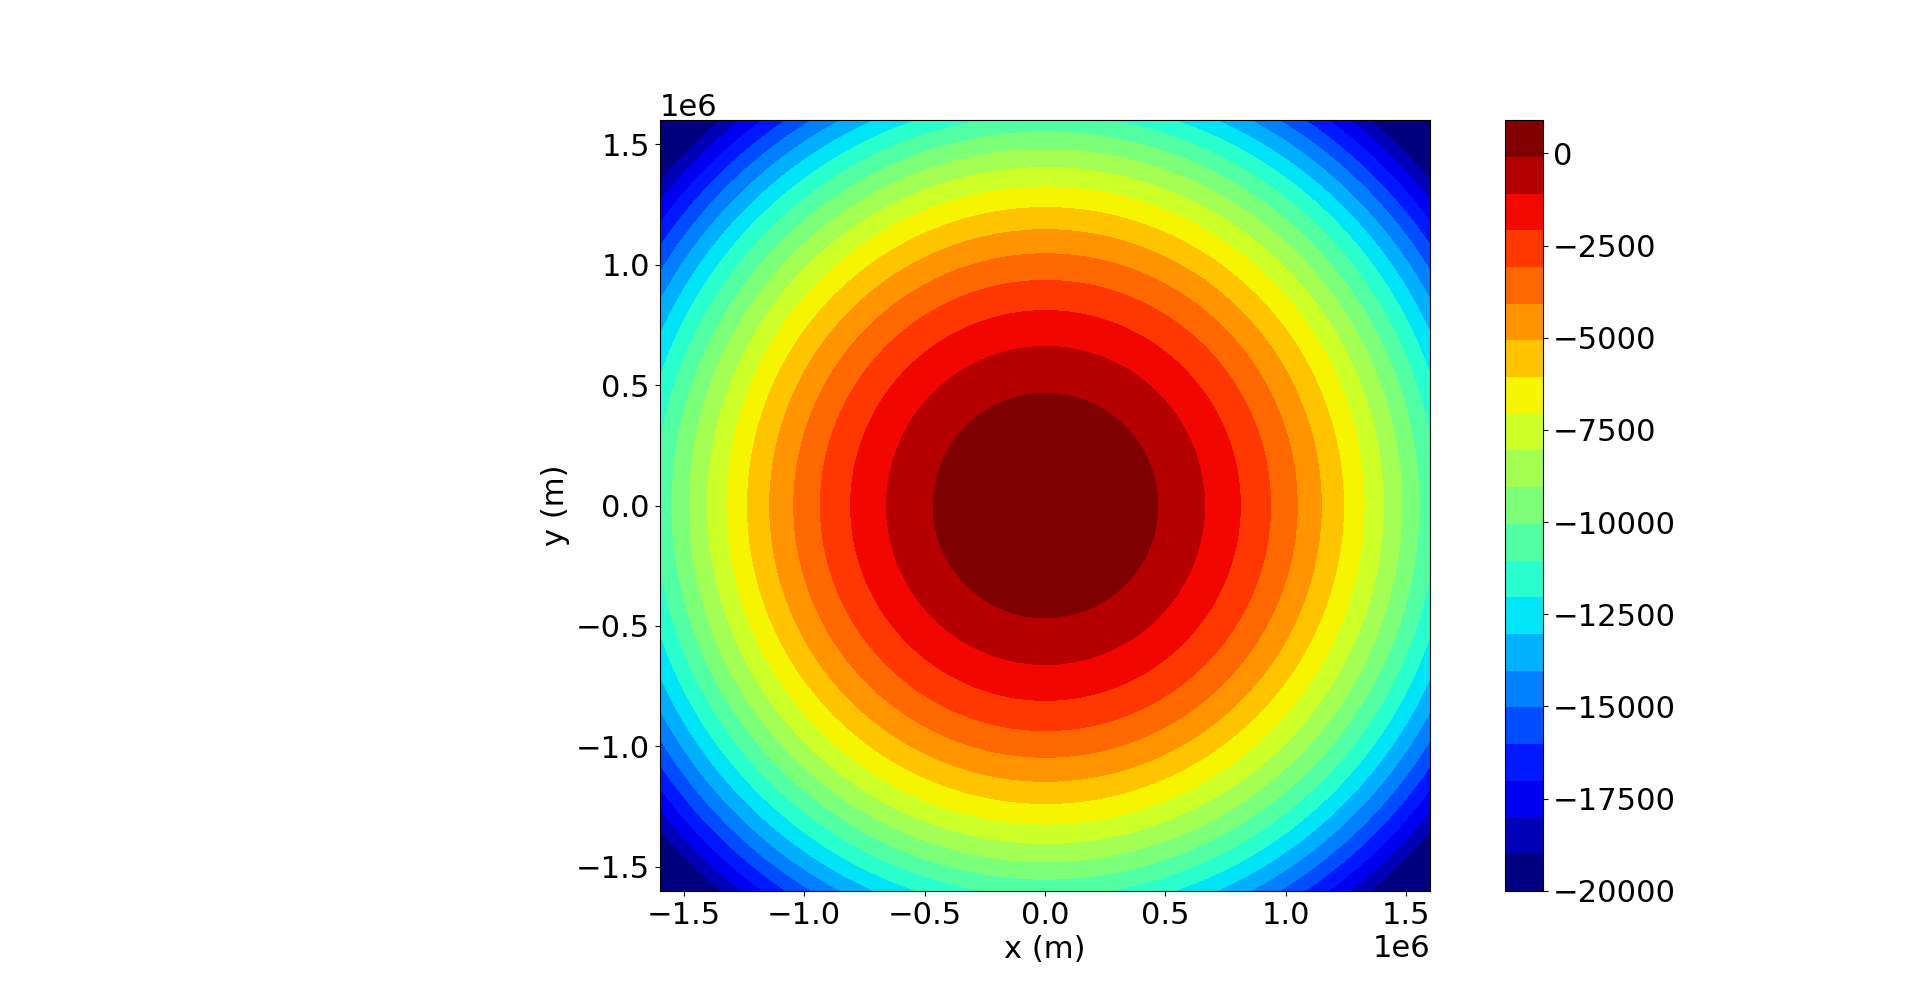
\includegraphics[width=0.7\linewidth]{../fig/circular_topo_top}
	\caption{Circular bedrock top view.}
	\label{circular_topo_top}
\end{figure}
\begin{figure}[!h]
	\centering
	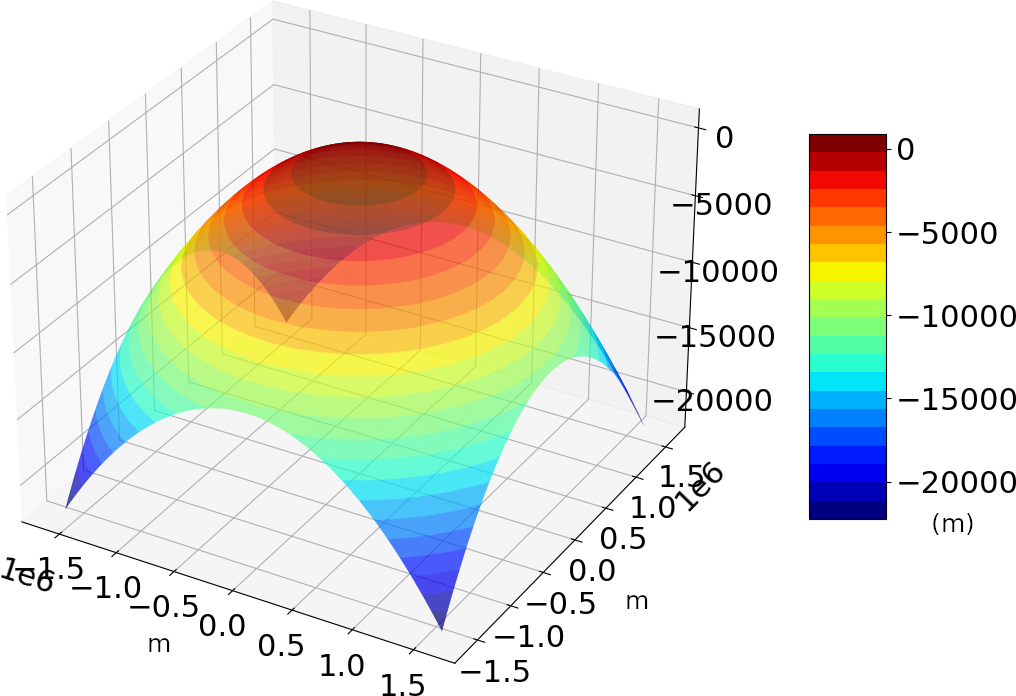
\includegraphics[width=0.7\linewidth]{../fig/circular_topo_jet}
	\caption{Circular bedrock sideview.}
	\label{circular_topo_jet}
\end{figure}
The thule bedrock configuration (Bed) is shown in Figure \ref{Thule_2D} and is given by:
\begin{equation}
	\theta=arctan2(y,x);
\end{equation}
\begin{equation}
	I=R-cos(2\theta)\frac{R}{2};
\end{equation}
\begin{equation}
	Bed_0=Bc-(Bc-BI)\frac{|x^2+y^2}{R^2};
\end{equation}
\begin{equation}
	Bed=Bacos(3\pi\frac{\sqrt[2]{x^2+y^2}}{I})+Bed_0;
\end{equation}
With $R=800 x 10^3 m$, $Bc=0,9 x 10^3 m$, $BI=-2 x 10^3 m$, and $Ba=1,1 x 10^3$.
\begin{figure}[!h]
	\centering
	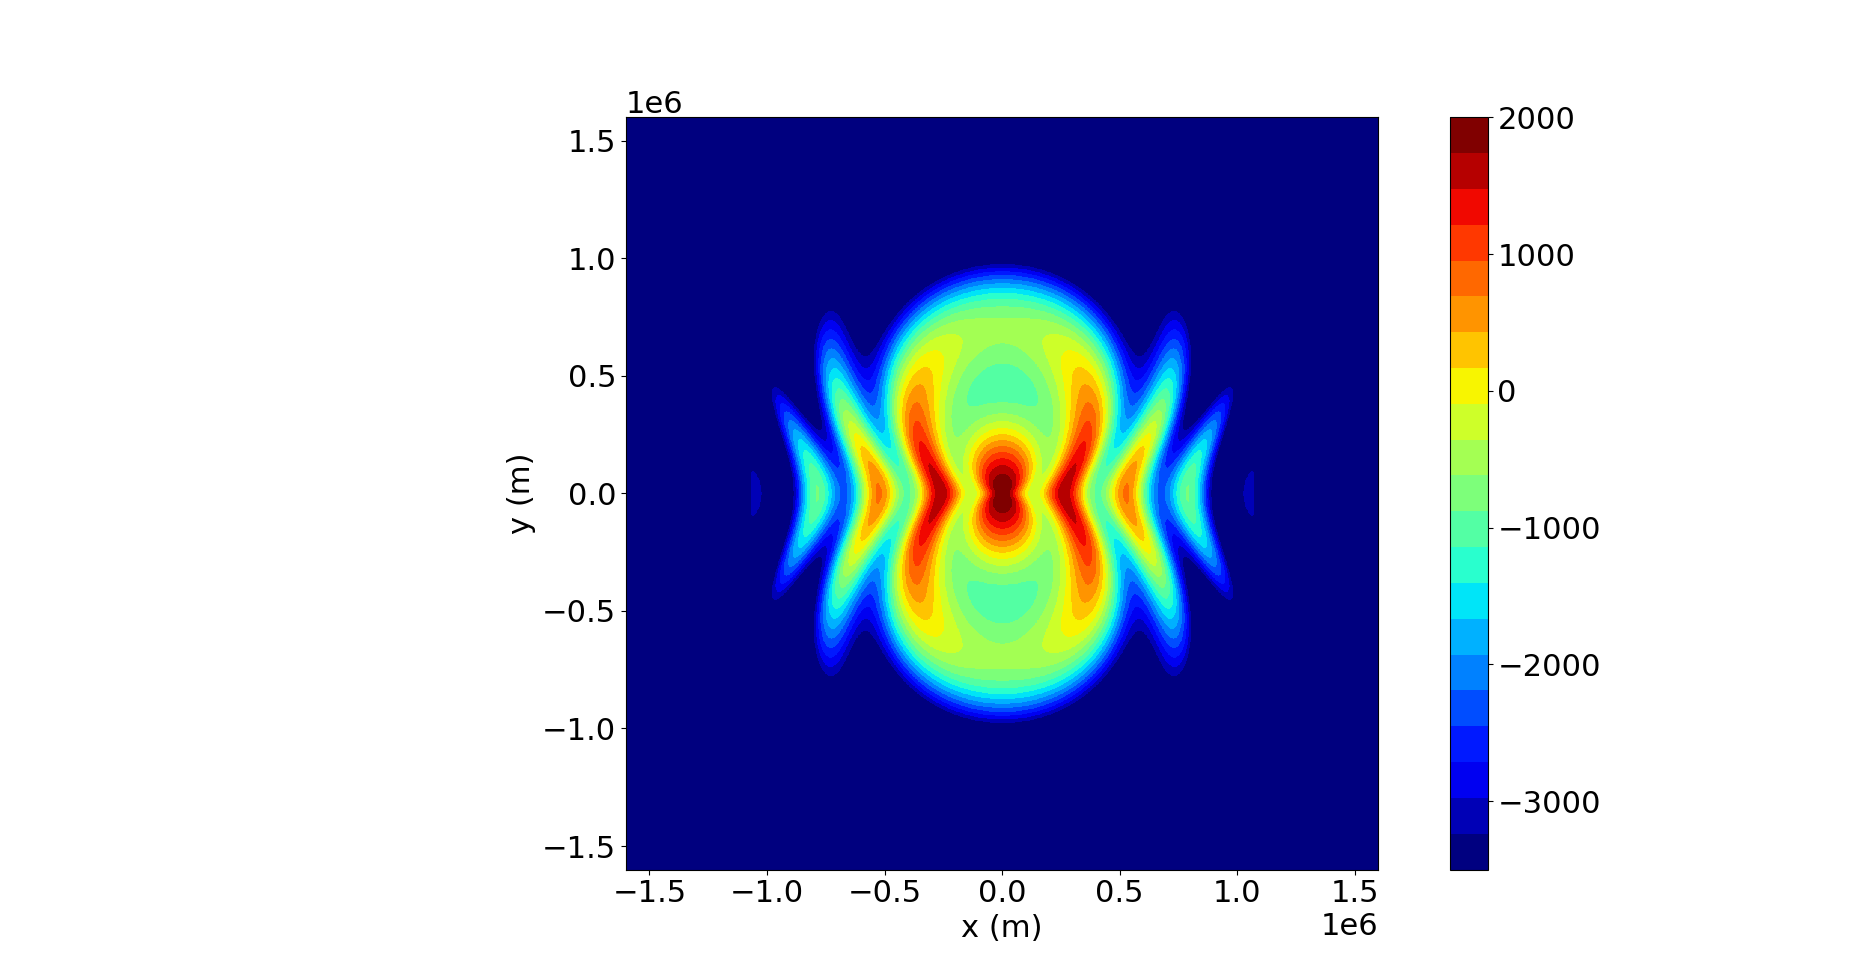
\includegraphics[width=0.7\linewidth]{../fig/Thule_2D}
	\caption{Thule bedrock topview.}
	\label{Thule_2D}
\end{figure}
\begin{figure}[!h]
	\centering
	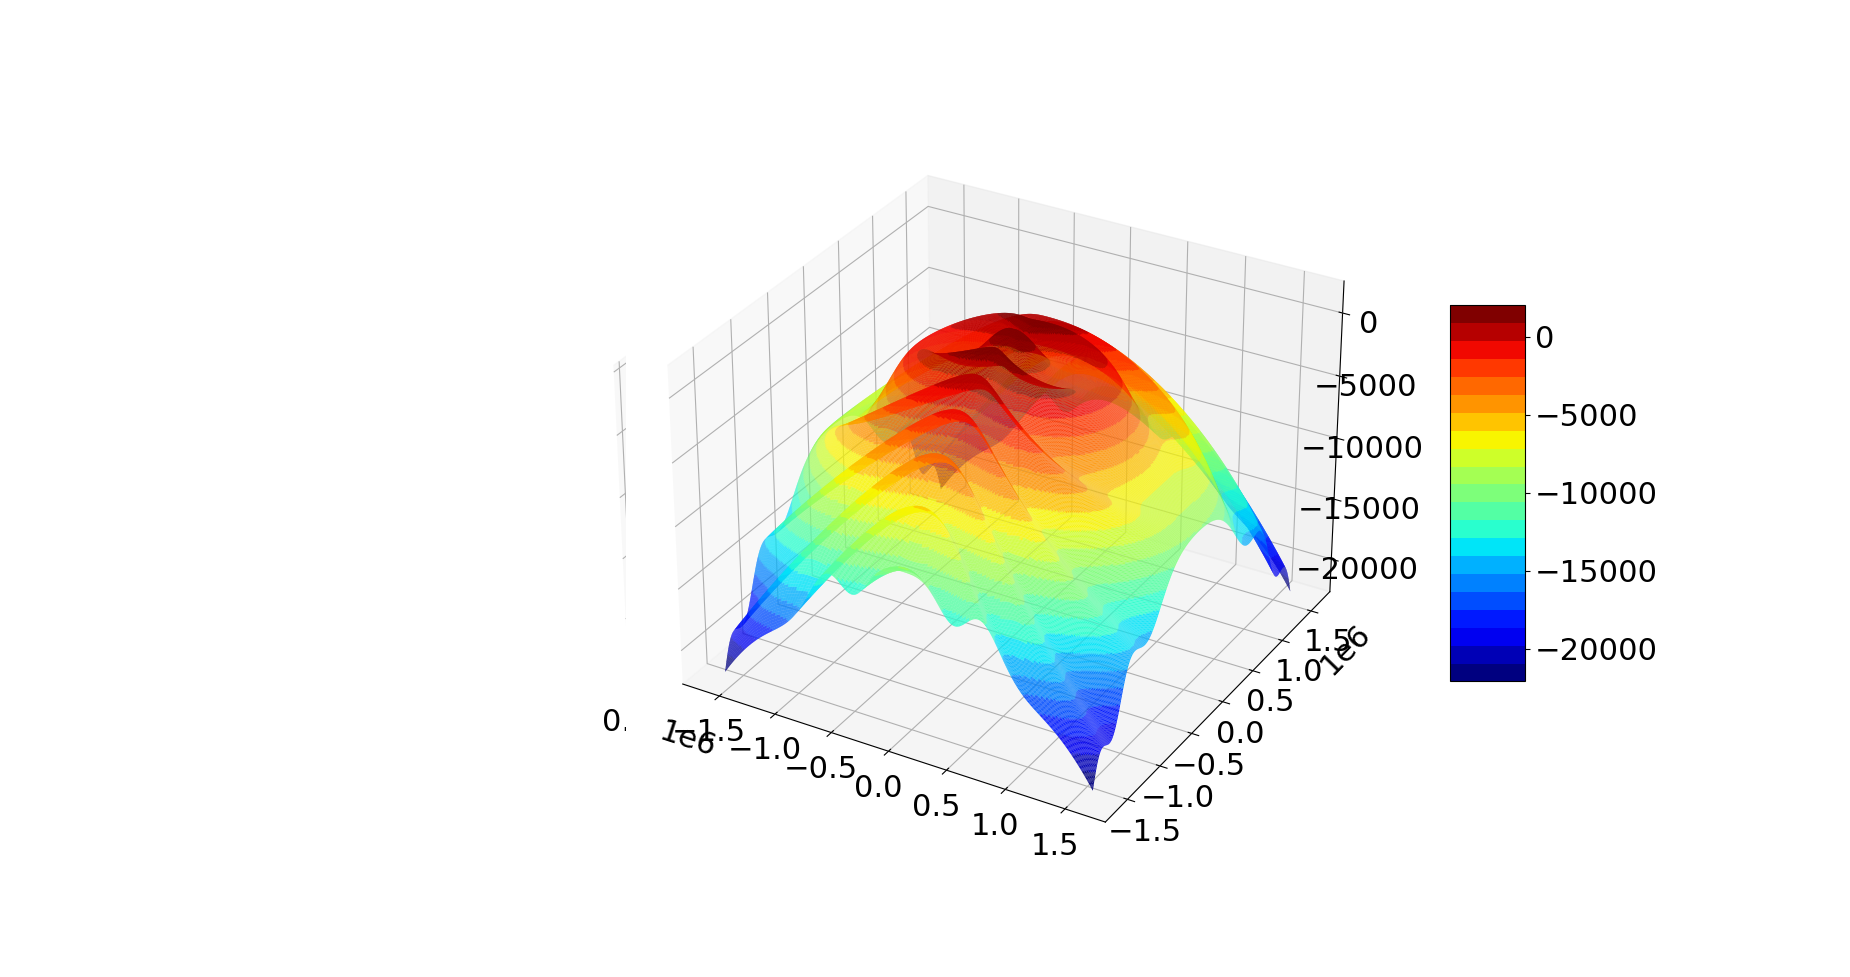
\includegraphics[width=0.7\linewidth]{../fig/Thule_3D}
	\caption{Thule bedrock topography 3D sideview.}
	\label{Thule_3D}
\end{figure}
\subsubsection{Boundary conditions}
Boundary conditions are needed in order to solve differential equations. It will be assumed that:
\begin{itemize}
	\item The bedrock is impermeable (The vertical component of the ice flow velocity is 0). 
	\item The flow follows Weertman friction law.
	\item Mass acumulation is a constant parameter.
	\item The simulation will be performed on a quarter of the domain, since the geometry of the topography is symmetric, which allows to have free slip boundary condition at the left and down side of the topography, and open boundary condition at the right and top side of the domain. 
\end{itemize}
\subsubsection{Physical parameters}
There will be two types of physical parameters in the simulation, the ones we will assume constant during all our simulations, and the ones which can vary during and in between the simulation. The figure \ref{Constants_parameters} presents the constant parameters that will be used
\begin{figure}[!h]
	\centering
	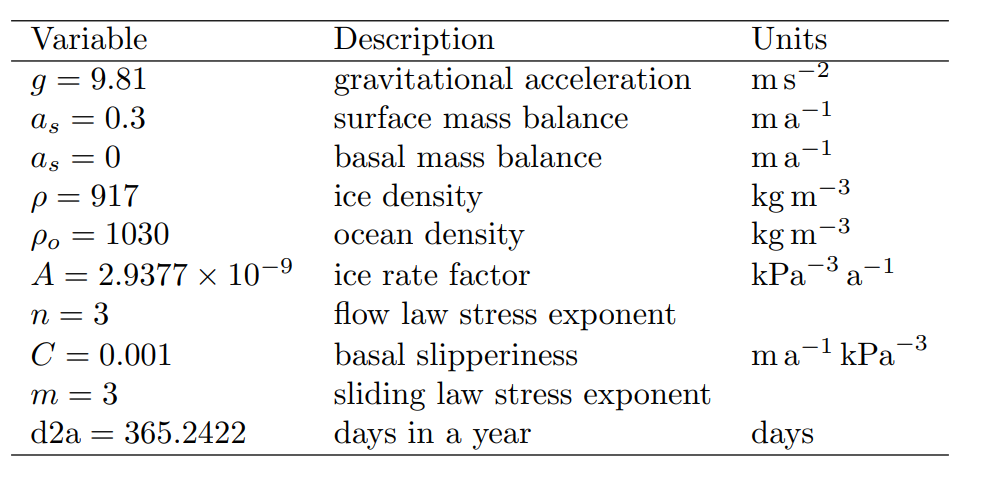
\includegraphics[width=0.7\linewidth]{../fig/Constants_parameters}
	\caption{Constants parameters based on Hilmar Gudmundsson's experiment for thule's configuration.}
	\label{Constants_parameters}
\end{figure}
The numerical resolution will be our variable physical parameter, which we will vary such that $\delta x= \delta y \in [0.250, 10] km$.
\subsubsection{External forcing}
We will assume that the only external force acting is the gravity ($g=9.81 m/s^2$), which is translated to the weight of the ice sheet and the flotation force of this in the ocean water.
\subsubsection{Initial condition}
The simulation starts from rest state, were no ice is formed. 
As stated before, the flow will follow the linear Weertman friction law at the base of the ice sheet:
\begin{equation}
	\tau_b=\beta u;
\end{equation}
Where $\tau$ is the friction shear stress, $\beta$ is the basal friction coefficient, and $u$ is the velocity.
Comparisons were made using friction coefficients ranging from $\beta=10^-8$ to simulate a friction close to 0, to $\beta=10^-2$. This coefficient is also the one chosen to perform the simulations. 
\subsubsection{Time step}
The Courant-Friedrichs-Lewy (CFL) condition is a necessary condition to solve numerically partial differential equations. It states that the distance a variable travels between two time steps must be smaller than the distance between two points of the mesh \cite[]{courant1967partial}. It is needed that:
\begin{equation}
	C=\frac{u\Delta t}{\Delta x}<Cmax;
\end{equation}
With C the courant number, $u$ the magnitude of the velocity, $\Delta t$ the time step, $\Delta x$ the horizontal resolution, and Cmax = 1. This implies then, for a given mesh:
\begin{equation}
	\Delta t < \frac{\Delta x}{u};
\end{equation}
This is a safe approximation. Cmax then has to be estimated running different parameters in the simulation and see if it converges or not. In order to satisfy the CFL condition, a good starting point is 1 year, since it works propertly and converges even for a resolution of 1km.
However, in this experiment it is asked to report the results every 10 years, and for this reason we will save the results of the simulation with a frequency of 10 years. 
\section{Tasks schedule}
Figure \ref{Schedule} shows the tasks schedule for the project, that will be held between the 12th of january 2023 and the 5th of may 2023. 
\begin{figure}[!h]
	\centering
	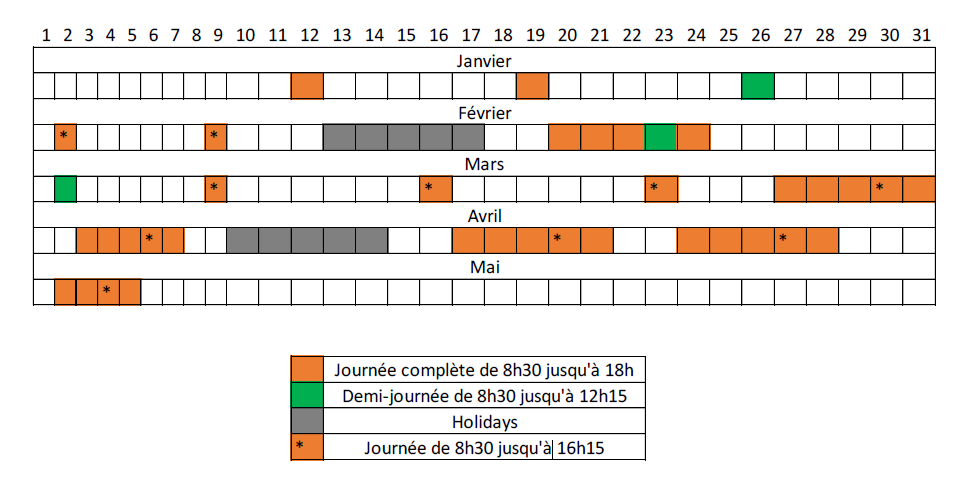
\includegraphics[width=0.7\linewidth]{../fig/Schedule}
	\caption{Tasks schedule.}
	\label{Schedule}
\end{figure}
The first two months, we will carry on the simulation of the first idealised case, for a circular topography. From february to march we will analyze the results from the first idealised case, and in the month of april we will carry on the simulation of the more realistic but still idealised thule topography. We will spend the last days of april analyzing the results of the lasts simulations and compare the results with different resolutions, to finally obtain a relation that allows us to see the change in the position of the grounding line, and working on the elaboration of the final report the first days of may. 
\bibliographystyle{jfm}
\bibliography{./biblio}
\end{document}
